\documentclass[11pt, oneside]{article} 
\usepackage{geometry}
\geometry{letterpaper} 
\usepackage{graphicx}
	
\usepackage{amssymb}
\usepackage{amsmath}
\usepackage{parskip}
\usepackage{color}
\usepackage{hyperref}

\graphicspath{{/Users/telliott_admin/Tex/png/}}
% \begin{center} 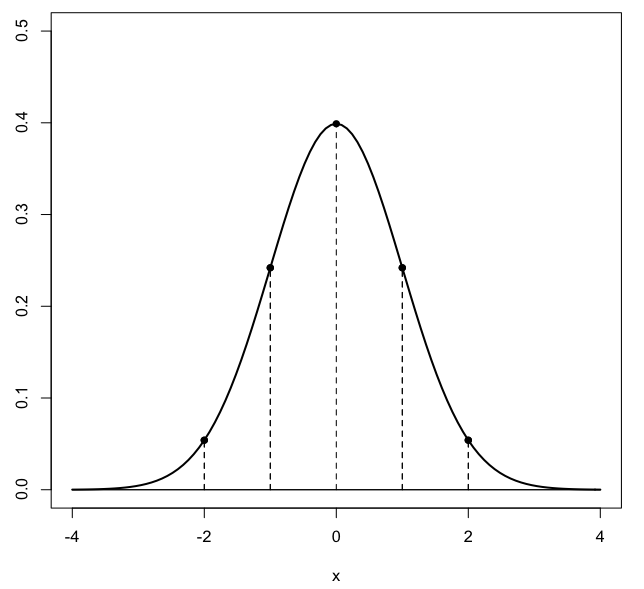
\includegraphics [scale=0.4] {gauss3.png} \end{center}

%break
\title{Another famous limit}
\date{}

\begin{document}
\maketitle
\Large
Consider the function of the variable $x$ defined by the power $b^x$, where $b$ is some arbitrary constant.
\[ f(x) = b^x \]

We will show later that the difference quotient whose limit defines $f'(x)$ can be manipulated to give the following form
\[ b^x \lim_{h \rightarrow 0} \frac{b^{h}-1}{h} \]

For this reason, we are interested in the properties of the limit
\[ \lim_{h \rightarrow 0} \frac{b^{h}-1}{h} \]

First, it is clear that the limit does not depend on $x$, so it is just a number.

\subsection*{working with the constant}

We can easily calculate the value of
\[ \lim_{h \rightarrow 0} \frac{b^{h}-1}{h} \]

Set $h=0.00001$ and use Python.  For the following values of $b$ I get:

$\circ$  $b=2$ gives $0.693$

$\circ$  $b=2.71828 \dots = e$ gives $1.000$

$\circ$  $b=10$ gives $2.303$

This gives us one \emph{definition} of $e$.  It is the value of $b$ for which this limit is equal to $1$.

It will not surprise you to learn that these values correspond to the natural logarithm of the base.

\subsection*{playing with the limit expression}

So starting from the definition that $e$ is the value for which
\[ \lim_{h \rightarrow 0} \frac{e^{h}-1}{h} = 1 \]

We can rearrange the equation as follows:
\[ \lim_{h \rightarrow 0} e^{h} = \lim_{h \rightarrow 0} 1 + h \]
\[ \lim_{h \rightarrow 0}  e = \lim_{h \rightarrow 0} (1 + h)^{1/h} \]
\[ e = \lim_{h \rightarrow 0} (1 + h)^{1/h} \]
since $e$ is just a constant (we haven't demonstrated that it is legal to manipulate limits in this way, but you can).

We can also substitute $nh = 1$ and so $n = 1/h$ and the expression can be written as
\[ e = \lim_{n \rightarrow \infty}  (1 + \frac{1}{n})^{n} \]
which is the first expression that we introduced for $e$.

All three limits are equivalent:
\[  e = \lim_{n \rightarrow \infty}  (1 + \frac{1}{n})^{n} \]
\[ =  \lim_{h \rightarrow 0} (1 + h)^{1/h} \]
and
\[  \lim_{h \rightarrow 0} \frac{e^{h}-1}{h} = 1 \]

We can calculate $e$ from this equation as well, but it doesn't converge so fast.  For $n=100000$, using Python, I got $e = 2.718168$, which is only correct to 3 decimal places.

On the other hand, one can use several approaches including the binomial theorem to evaluate 
\[ e = \lim_{n \rightarrow \infty} (1 + \frac{1}{n})^{n} \]
and show that it is equivalent to
\[ e = \frac{1}{0!} + \frac{1}{1!} + \frac{1}{2!} + \frac{1}{3!} + \cdots  \]
which is yet another one of the many definitions for $e$.

The first three terms are $1 + 1 + 1/2$, which is reasonably close. After six terms, we have $e = 2.718$.  The series converges rapidly because the inverse factorials get small very quickly.
We calculate $e$ as about $2.71828$.

\subsection*{the function}
In general we are interested in the \emph{function} $e^x$ and not just the number $e$.  

Start with a general exponential (base $b$) and consider the problem of finding its slope.  We want to see what happens to the exponential function when we vary $x$ by a small amount $h$.  

We want the difference quotient
\[ \lim_{h \rightarrow 0} \frac{b^{x+h} - b^x}{h} \]

for some unspecified base $b$.  We can rewrite this as
\[ \lim_{h \rightarrow 0} \frac{b^{x}(b^{h}-1)}{h} \]

The great insight is to note that $b^x$ does not depend on $h$, so it doesn't change as we go to the limit, and thus we have
\[ b^x \lim_{h \rightarrow 0} \frac{b^{h}-1}{h} \]

the limit is not dependent on $x$, so it is a constant.  Therefore, the slope of the exponential
\[ y = b^x \]
for some base $b$ is
\[ y' = cb^x \]
The slope is the same as the function, up to a constant.  

\subsection*{the exponential function}

The number $e$ is such that if $b=e$, then $c=1$ and we will have:
\[ y = e^x \]
\[ y' = e^x \]

The function $e^x$ is its own derivative, which leads to all of its amazing properties.

Write
\[ e^x = \lim_{n \rightarrow \infty} \ [ \ (1 + \frac{1}{n})^{n} \ ]^x \]
\[ e^x = \lim_{n \rightarrow \infty} \ (1 + \frac{1}{n})^{nx} \]

It turns out this is exactly the same as
\[ = \lim_{n \to \infty} (1 + \frac{x}{n})^{n} \]
which seems counterintuitive.  

But the result follows from
\[ (1+b)^{mn} = (1+mb)^n \]

\subsection*{a quick proof}

We saw this proof in the previous chapter.  We want to show that
\[ \lim_{n \rightarrow \infty} (1 + \frac{r}{n})^{n}  = \lim_{n \rightarrow \infty} \ [ \ (\frac{1}{n})^{n} \ ] ^r \]
Start with
\[ \lim_{n \rightarrow \infty} (1 + \frac{r}{n})^{n}  = \lim_{n \rightarrow \infty} (1 + \frac{r}{n})^{(n/r)r} \]

Define $m = n/r$ and so as $n \rightarrow \infty$, so does $m \rightarrow \infty$ and then we have
\[ \lim_{m \rightarrow \infty} (1 + \frac{1}{m})^{(m)r} \]
and the $r$ is outside.  $m$ is just a dummy variable so we write:
\[ \lim_{n \rightarrow \infty} \ [ \  (1 + \frac{1}{n})^{n} \ ]^r \]

$\square$

\subsection*{proof using the binomial}

Write the binomial expansion for both versions.  For the first, we have
\[ (1+b)^{mn} = 1 + (mn)b + \frac{(mn)(mn-1)}{2!} b^2 + \frac{(mn)(mn-1)(mn-2)}{3!} b^3 + \dots \]
In the limit as $n \rightarrow \infty$, the subtracted values of $k = 1,2,3 \dots$ are negligible and we have
\[ = 1 + (mnb) + \frac{1}{2!} (mnb)^2 + \frac{1}{3!} (mnb)^3 + \dots \]
For the second we get
\[ (1+mb)^n = 1 + n(mb) + \frac{n(n-1)}{2} (mb)^2 + \frac{n(n-1)(n-2)}{3!} (mb)^3 + \dots \]
and with the same limit, we get the identical formula.

Going back to
\[ e^x = \lim_{n \to \infty} (1 + \frac{x}{n})^{n} \]

\[ = \frac{1}{0!}(\frac{x}{n})^0 + + \frac{n}{1!}({\frac{x}{n}})^1 + \frac{n(n-1)}{3!}({\frac{x}{n}})^2 + \frac{n(n-1)(n-2)}{3!}({\frac{x}{n}})^3 + \cdots  \]

The $n$'s cancel and we have
\[ e^x = \frac{x^0}{0!} + \frac{x^1}{1!} + \frac{x^2}{2!} + \frac{x^3}{3!} + \cdots \]
\[ = 1 + x + \frac{x^2}{2!} + \frac{x^3}{3!} + \cdots  \]

This approach assumes that the binomial applies to fractional exponents, which is a bit complicated to show.

$\square$

\subsection*{sketch of a proof using Taylor series}

A more sophisticated way to do this is to use Taylor series, together with the fact that the derivative of $e^x$ is equal to $e^x$.

We can find the value of $e^x$ near $x=0$ as
\[ e^x = \sum_{n=0}^{n=\infty} \ \frac{f^n(0)}{n!} x^n \]

In particular, all the derivatives are just $e^x = 1$ at $x = 0$ so
\[ e^x = \sum_{n=0}^{n=\infty} \ \frac{x^n}{n!} \]
\[ = \frac{x^0}{0!} + \frac{x}{1!} + \frac{x^2}{2!} + \frac{x^3}{3!} \dots \]

and if $x=1$ we have that
\[ e^1 = e = 1 + 1 + \frac{1}{2!} + \frac{1}{3!} \dots \]

\subsection*{The exponential is its own derivative}

As we've emphasized, the most important fact about the exponential function $f(x) = e^x$ is that this function is its own derivative.  

Above, we derived the famous series for
\[ e^x = \sum_{n=0}^{\infty} \frac{x^n}{n!} = \frac{x^{0}}{0!} + \frac{x^{1}}{1!} + \frac{x^{2}}{2!} + \cdots  \]

Note that a good approximation for small $x$ is
\[ e^x \approx 1 + x \]

If you need more precision, you can add another term:
\[ e^x \approx 1 + x + \frac{x^2}{2!} \]

It is easy to see that the derivative of this series is the series itself.

Take $\frac{d}{dx}$ of the last series.

\[ \frac{d}{dx} \ e^x = 0 + (1)\frac{x^{1-1}}{1!} + (2)\frac{x^{2-1}}{2!} + (3)\frac{x^{3-1}}{3!} + \cdots  \]
\[ \frac{d}{dx} \ e^x = 0 + \frac{x^{0}}{0!} + \frac{x^{1}}{1!} + \frac{x^{2}}{2!} + \cdots  \]
\[ = e^x \]
Each exponent $n$ that comes down through the power rule, finds an $n$ in $n!=n \times (n-1) \times (n-2) \dots $ to cancel, leaving $n-1$ in the exponent as well as $(n-1)!$.


\end{document}